\chapter{Network Layer}
\label{chapter:networklayer}

This section explains the network layer and describes how its responsiblites were designed and implemented.

The network layer is the bottom layer in the 3 layer architecture of ACE. The network layer is responsible for all communication issues between running instances of ACE that are connected by communication networks. The core responsiblities are:

\begin{itemize}
 \item automatic user discovery in the local area network
 \item explicit user discovery on the Internet
 \item document management communication
 \item collaborative editing session communication
\end{itemize}

The network layer can be viewed as the interface between the physical network and the collaboration layer. Therefore, all messages received from the physical network are appropriately processed and passed to the collaboration layer. The network layer is not aware of the application layer.

Basically, the network layer provides core functionality independent of the activity of the user. Besides, depending on the activity of the user, being either participant or publisher of a document session, the network layer provides a client specific part (participant part) and a server specific part (publisher part).


\section{Overview}

This section gives a high-level overview about the network layer design and implementation by using two different point of views.

\subsection{Architecture}

The figure depicts the rough architecture of the network layer. The collaboration layer interacts only with the \texttt{Net} component. Through this component, the collaboration layer either accesses the \texttt{Protocol} component or the \texttt{Core} component. The latter interacts with the \texttt{Discovery} component as well as with the \texttt{Protocol} component. The \texttt{Protocol} accesses the \texttt{BEEP} framework whereas the \texttt{Discovery} accesses the \texttt{DNSSD} service.

\begin{figure}[H]
 \centering
 \frame{
 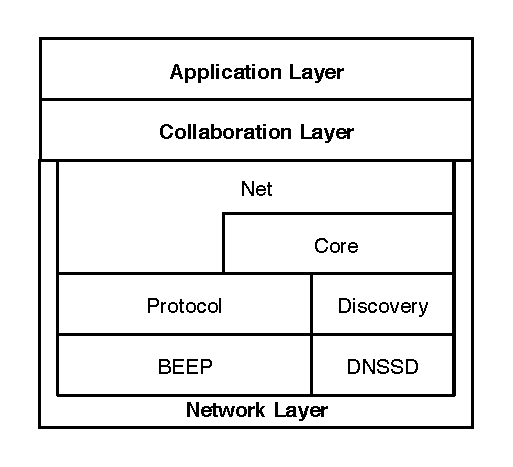
\includegraphics[width=4.18in,height=5.64in]{../images/finalreport/network_architecture_view.eps}
 }
 \caption{Network Layer Architecture}
 \label{fig:network.architecture}
\end{figure}


\subsection{Packages}

The top level package \texttt{net} contains all the interfaces through which the collaboration layer and the network layer interact. All other packages in the network layer are subpackages of the \texttt{net} package. The \texttt{core} package provides core classes to the network layer and contains default implementations for several interfaces declared in the \texttt{net} package. It depends on the \texttt{protocol} and the \texttt{discovery} packages.

The \texttt{discovery} package contains the relevant functionality for dynamic user discovery as well as user management. It has a subpackage \texttt{dnssd} which contains DNSSD specific classes. The \texttt{discovery} and the \texttt{dnssd} packages interact with the DNSSD component.

The \texttt{protocol} package implements all communication related functionality and directly interacts with the BEEP component. The subpackage \texttt{filter} contains classes for the processing of outgoing and incoming requests and messages, respectively.

\begin{figure}[htb]
 \centering
  \frame{
 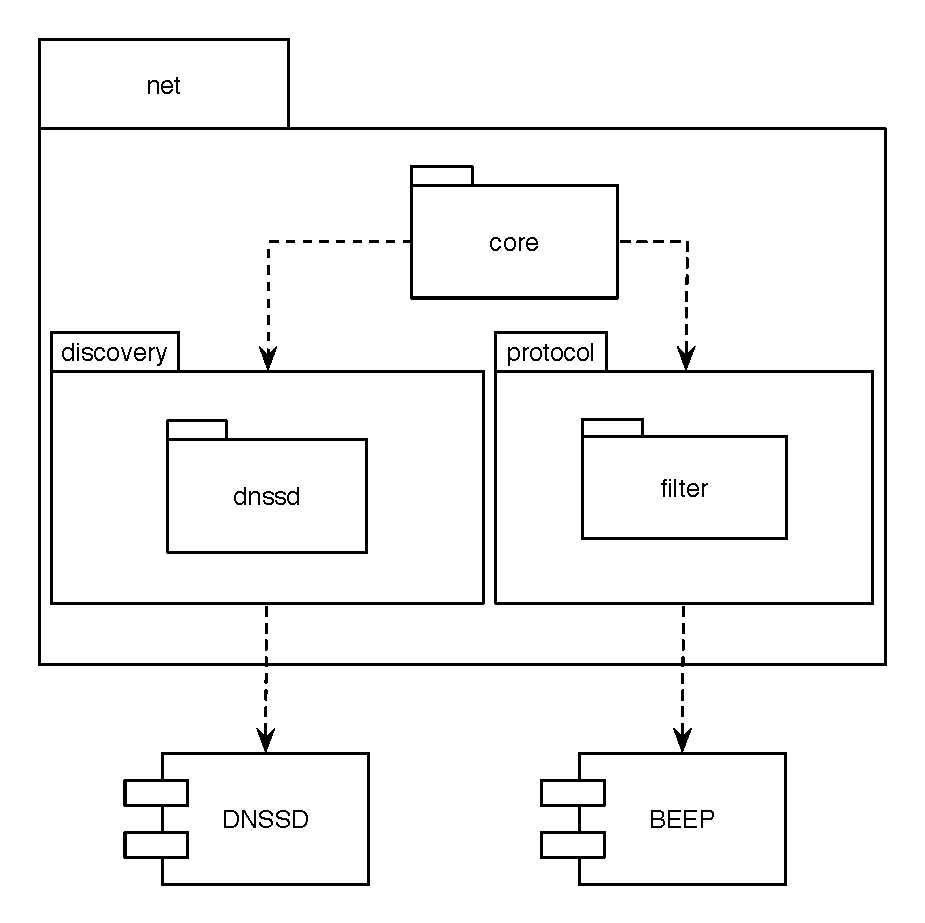
\includegraphics[width=5.94in,height=5.93in]{../images/finalreport/network_package_view.eps}
 }
 \caption{Network Layer Package Structure}
 \label{fig:network.architecture}
\end{figure}


\section{User Discovery component}
This section explains the implemented solution for the dynamic and automatic user discovery in greater detail.

\subsection{Responsabilities}
The user discovery takes over the task of discovering all possible user events in the local area network. This includes the dynamic discovery of new users, the leaving of users and the notification of metadata changes for a particular user. Currently, the user's metadata subject to change adds up to the user's name only but could be extended easily for more values.

The user discovery component must meet the following core requirements:

\begin{itemize}
 \item notification about new discovered users
 \item deliver full address information for each discovered user
 \item notification about discarded users
 \item notification about user detail changes
 \item start and stop possiblity for the discovery process 
\end{itemize}

These requirements could be met by multiple technologies. We decided that Bonjour zero-conf networking technology would best meet our requirements. Please read the chapter ????? for a justification on that decision.

\subsection{Design}
\subsubsection{Client view of the discovery component}
The first step on the design was to find a way to use the discovery component independent of its implementation. That is, to have a transparent discovery usage for the client, without him knowing the concrete implementation. This consideration is in line with the general design principle of ACE to have an architecture with interchangeable components.

\begin{figure}[H]
 \centering
  \frame{
 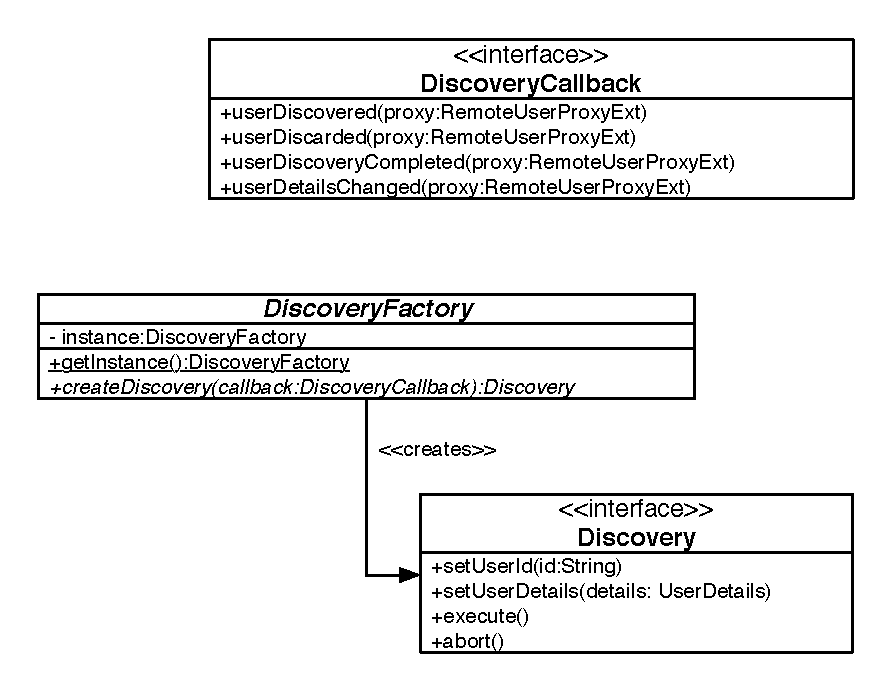
\includegraphics[width=5.72in,height=4.39in]{../images/finalreport/network_discovery_uml.eps}
 }
 \caption{Discovery usage design}
 \label{fig:network.discovery.usage}
\end{figure}

The abstract class  \texttt{DiscoveryFactory} provides the entry point for a client who wants to use the discovery service. To create a new  \texttt{Discovery}, a  \texttt{DiscoveryCallback} implementation must be passed. This implementation is provided by the client to the discovery component. All events received from the network by the discovery are finally given to that callback. The  \texttt{Discovery} type enables the client to set the  essential information for the local user and to start and stop the discovery service.

This design makes the concrete discovery implementation (i.e. the technology used) transparent to the client.


\subsubsection{DiscoveryManager}
The  \texttt{DiscoveryManager} plays a major role in the discovery component. It keeps track of all active users (who have not been discarded) and their session states (established/not established). All user management is done through this class. So each other component of the network layer falls back on the  \texttt{DiscoveryManager} if user bookkeeping needs to be done.

All events that the discovery receives are first processed in collaboration with the \texttt{DiscoveryManager} implementation before they are passed to the  \texttt{DiscoveryCallback}.

\begin{figure}[H]
 \centering
  \frame{
 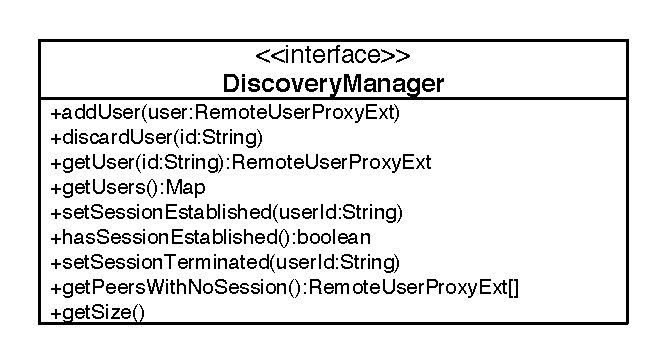
\includegraphics[width=4.22in,height=2.19in]{../images/finalreport/network_discoveryManager_uml.eps}
 }
 \caption{Discovery Manager}
 \label{fig:network.discovery.manager}
\end{figure}


\subsubsection{DNSSD calls}
\texttt{DNSSDCall} is an abstract base class for all DNSSD API calls. A subclass defines what API call is executed. \texttt{DNSSDCall} incorporates advanced \texttt{Exception} and \texttt{Error} handling. That is, in case of failure, it uses a \texttt{RetryStrategy} to determine how many times and in what intervals a call is repeated. If the retry strategy fails, the exception is reported to the upper layer and the discovery process aborted (See section Exception Handling for further details???????). The \texttt{DNSSDCall} design follows the command pattern (see [Design Patterns]) in that each call is wrapped by a command object and can uniformly be executed.

\begin{figure}[H]
 \centering
  \frame{
 
\includegraphics[width=2.97in,height=1.08in]{../images/finalreport/network_dnssdCall_uml.eps}
 }
 \caption{DNSSDCall abstract super class}
 \label{fig:network.discovery.manager}
\end{figure}


\subsection{Implementation}
This section outlines how the concrete discovery implementation with Bonjour was designed and implemented. The design was lead by the listener oriented API of Bonjour (see ????? for further details on this technology).

\subsubsection{Bonjour discovery}
The concrete \texttt{Discovery} implementation is called \texttt{Bonjour} and is created by the \texttt{BonjourFactory} factory. Class \texttt{Bonjour} starts and stops the discovery process with Bonjour zero-conf networking technology. For this purpose,  \texttt{Bonjour} makes use of two further types:  \texttt{UserRegistration} and \texttt{PeerDiscovery}.

\begin{figure}[htb]
 \centering
  \frame{
 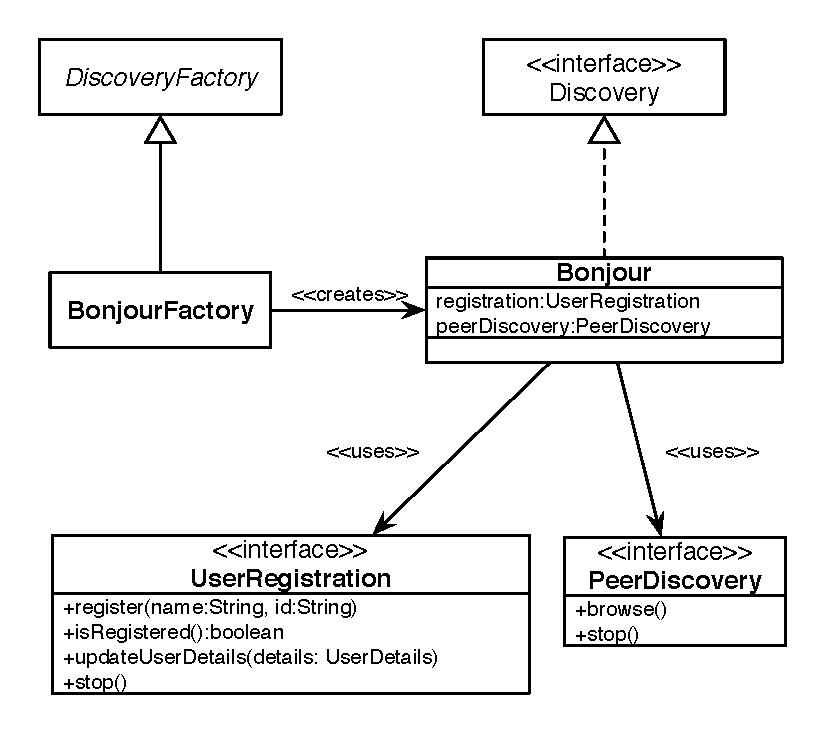
\includegraphics[width=5.28in,height=4.67in]{../images/finalreport/network_bonjour_uml.eps}
 }
 \caption{Discovery Implementation}
 \label{fig:network.discovery.implementation}
\end{figure}

\paragraph{User Registration}
 \texttt{UserRegistration} allows to register the local user for discovery as well as to update the user's details. It extends 
 various listener interfaces specified by the DNSSD API, namely  \texttt{RegisterListener},  \texttt{ResolveListener} and  \texttt{QueryListener}. This allows to have the user registration process separate from the peer discovery process, which uses the same listener interfaces. Consider figure \ref{fig:network.discovery.userregistration}.

\begin{figure}[H]
 \centering
  \frame{
 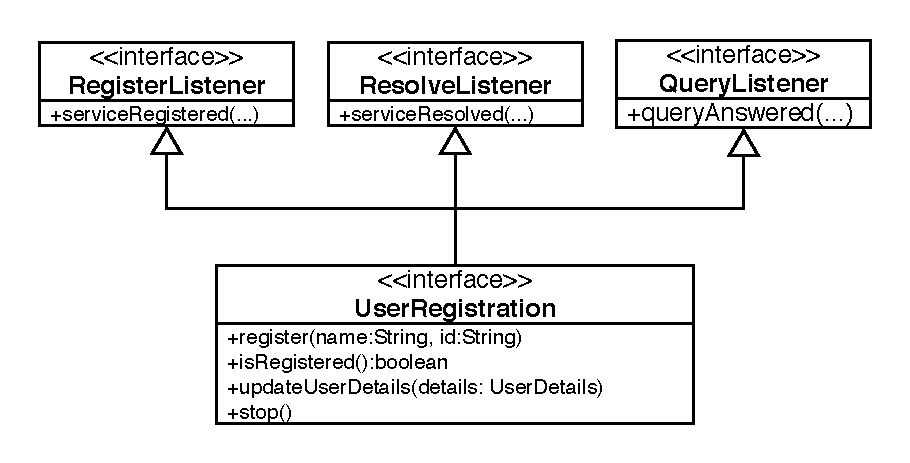
\includegraphics[width=5.85in,height=2.86in]{../images/finalreport/network_userRegistration_uml.eps}
 }
 \caption{User Registration and extended interfaces}
 \label{fig:network.discovery.userregistration}
\end{figure}


\paragraph{Peer Discovery}
\begin{figure}[H]
 \centering
  \frame{
 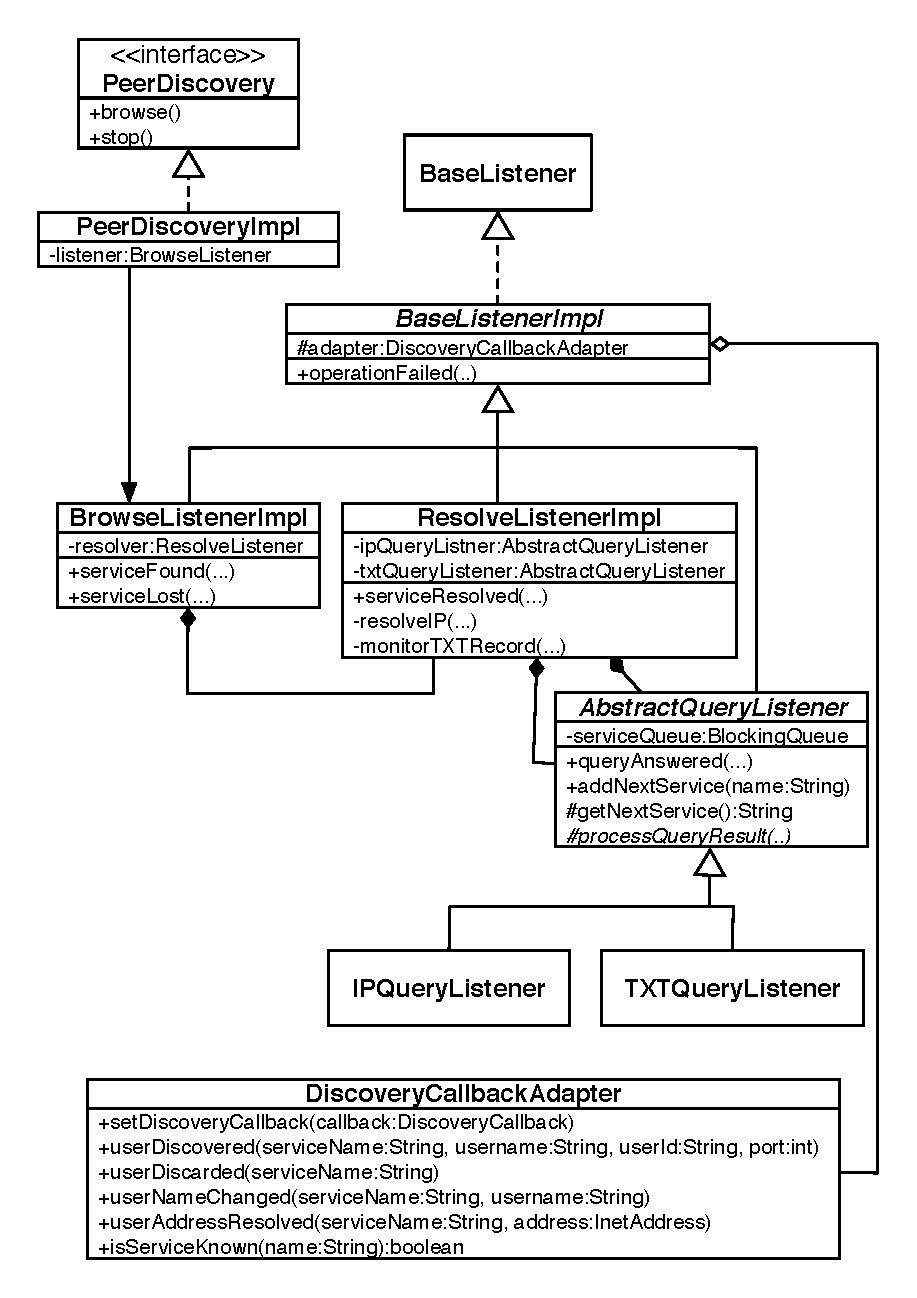
\includegraphics[width=5.89in,height=8.43in]{../images/finalreport/network_peerDiscovery_uml.eps}
 }
 \caption{Peer Discovery Design and Implementation}
 \label{fig:network.discovery.peerdiscovery}
\end{figure}

\texttt{PeerDiscovery} allows for the discovery of peer users who reside on the same local area network (this constraint is   imposed by the Bonjour technology). The \texttt{PeerDiscovery} implementation has a reference to the \texttt{BrowseListenerImpl} class. It receives browse events from the DNSSD component (service found, service lost). When a new service (i.e. user) was found, \texttt{BrowseListenerImpl} starts a new DNSSD call to resolve that service (i.e. receive TXT record with specific information for that user). The call is passed a reference to \texttt{ResolveListenerImpl}, which will receive the results of that call (see also section on DNSSD calls ??????). On the other side, a serviceLost event is directly forwarded to the \texttt{DiscoveryCallbackAdapter} (see below for a description of that class). 

\texttt{ResolveListenerImpl} handles serviceResolved events. It first forwards the event to the \texttt{DiscoveryCallbackAdapter} and second starts two further DNSSD calls for the IP address resolving of the discovered user and the monitoring for the user's TXT record (i.e. to be notified when that user changes its TXT record, e.g. his name).

The listeners for the two DNSSD calls are \texttt{IPQueryListener} and \texttt{TXTRecordListener}. Both extend the \texttt{AbstractQueryListener}. Their functionality is straightforward: The events are simply forwarded to the \texttt{DiscoveryCallbackAdapter}.

The \texttt{DiscoveryCallbackAdapter}, as its name suggets, is an adapter for all listeners to forward their DNSSD events. This class allows to have a central place where all events from the DNSSD discovery are gathered and uniformly processed. The implementation of this interface \texttt{DiscoveryManagerImpl} also implements \texttt{DiscoveryManager} and represents the central processing place for events from the discovery side as well as the user management handler the remaining network layer part.

\begin{figure}[H]
 \centering
  \frame{
 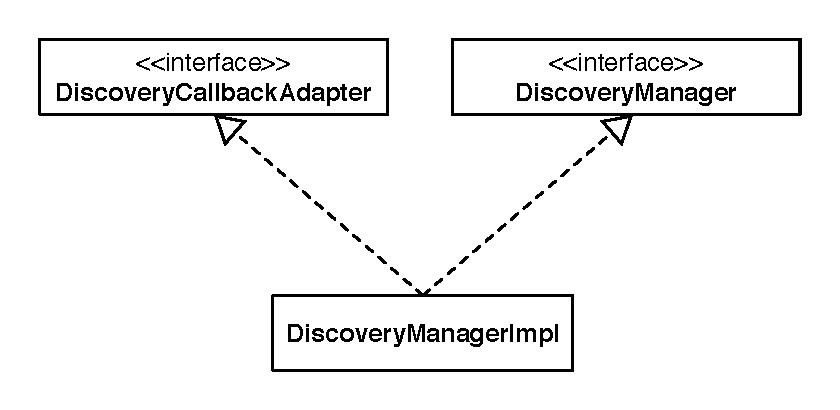
\includegraphics[width=5.38in,height=2.51in]{../images/finalreport/network_discoveryManagerImpl_uml.eps}
 }
 \caption{Discovery Callback Adapter and Discovery Manager Implementation}
 \label{fig:network.discovery.managerandadapter}
\end{figure}


\paragraph{Concrete DNSSD calls}
There are various implementations for the abstract super class \texttt{DNSSDCall}, including \texttt{Register}, \texttt{Browse}, \texttt{Resolve}, \texttt{QueryRecord} and \texttt{TXTUpdate}.

\begin{figure}[H]
 \centering
  \frame{
 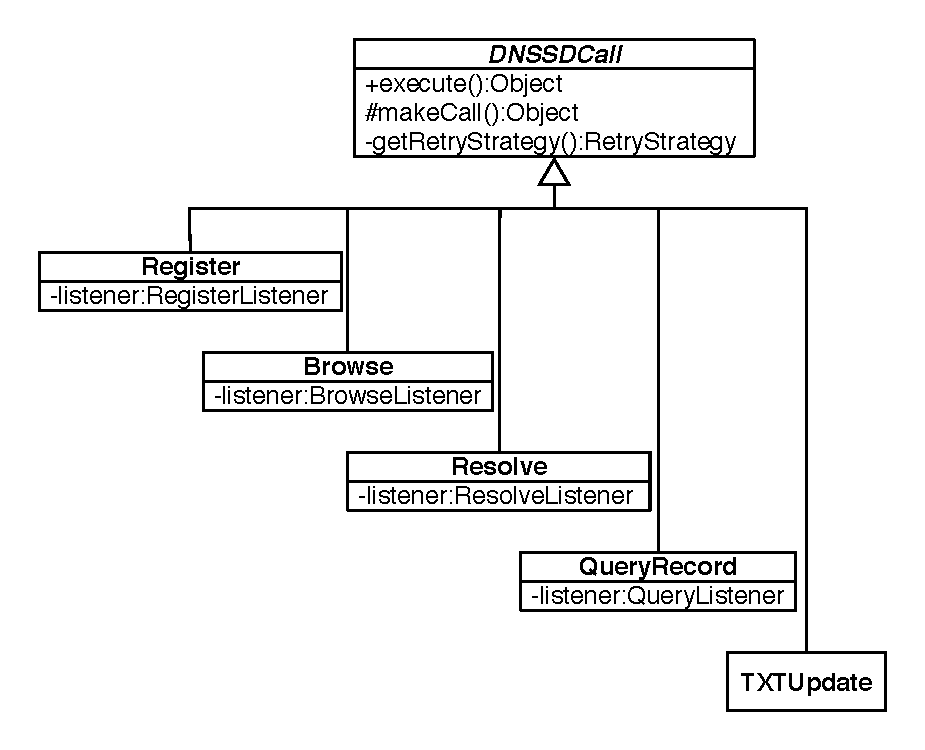
\includegraphics[width=5.94in,height=4.78in]{../images/finalreport/network_dnssdCall_impl_uml.eps}
 }
 \caption{DNSSDCall implementations}
 \label{fig:network.discovery.manager}
\end{figure}

\subsection{Explicit user discovery}
TODO!!!!!!

\subsection{Use cases}
\subsubsection{Start of discovery process}
The following sequence diagram shows how the client uses the discovery and what happens behind the \texttt{execute()} call.

\begin{figure}[H]
 \centering
  \frame{
 \includegraphics[width=5.90in,height=5.76in]{../images/finalreport/network_discovery_sequence.eps}
 }
 \caption{Launch of the Discovery Process}
 \label{fig:network.discovery.launch}
\end{figure}

%if time, add more use cases

\subsection{Exception handling}
All necessary exception handling is captured in \texttt{DNSSDCall} and in \texttt{BaseListenerImpl}. 

\texttt{DNSSDCall} catches exceptions and retries the DNSSD call as long as the \texttt{RetryStrategy} determines. If the retry strategy fails, the exception is reported to the upper layer and the discovery process aborted. If the first executed DNSSD call throws an \texttt{Error}, then this is interpreted that the DNSSD (Bonjour) is not installed on the local host. The discovery process is aborted and the upper layer notified.

\texttt{BaseListenerImpl} implements an exception method \texttt{operationFailed(...)} which must be available for all DNSSD listeners. If this method is called, it is interpreted as an unrecoverable error. Thus, the upper layer gets reported and the discovery process aborted.

\subsubsection{Retry Strategy}
The retry strategy design shall give an advanced exception handling and some way of service recovery in that calls are retried a certain number of times. The retry strategy determines how long the executing thread should wait untill it retries to execute the DNSSD call. If the call fails again, the retry strategy is asked again how long the thread should wait untill the next call. If the retry strategy fails, it throws an exception to indicate that the thread should stop retrying the DNSSD call and abort. This strategy could be applied for all network related method calls, but yet it is used only for DNSSD calls. 

\begin{figure}[H]
 \centering
  \frame{
 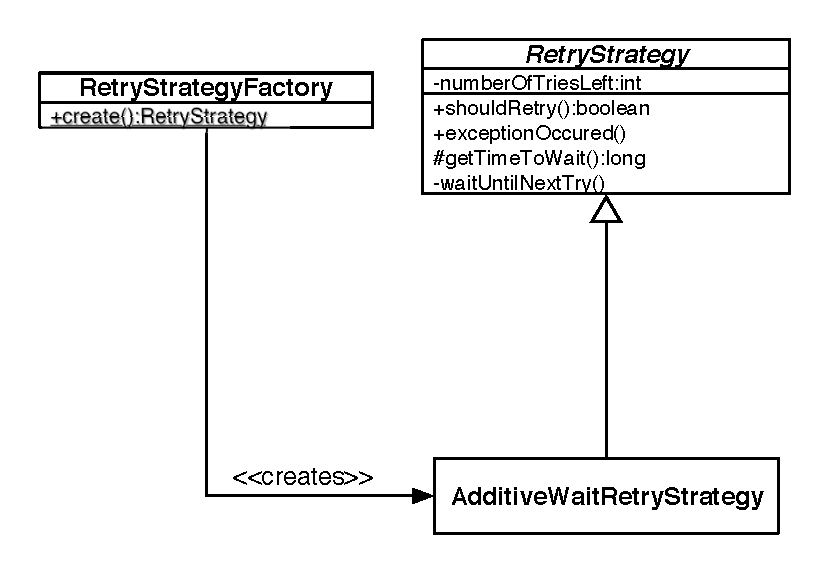
\includegraphics[width=5.31in,height=3.60in]{../images/finalreport/network_retryStrategy_uml.eps}
 }
 \caption{Retry Strategy Design and Implementation}
 \label{fig:network.discovery.retrystrategy}
\end{figure}

The \texttt{AdditiveWaitRetryStrategy} can be configured to start with an initial waiting time and an increment wait time for succeeding retries. So for example, if the initial waiting time is 3 seconds and the increment wait time is 2 seconds, the executing thread of the DNSSD call will wait for 3 seconds after the first failed execution of the call, and 5 seconds after the second time and so on untill the strategy throws a \texttt{RetryException} indicating that the thread should abort retrying.

% end documentation of user discovery


\section{Communication component}
This section describes the design and the implementation of the communication component in greater detail. Henceforth, a basic knowledge of the Java BEEP core library is expected in order to understand the explanations. See section ?????????? for an introduction on BEEP.

\subsection{Responsabilities}
The communcation component is responsible for all communication between the peers and users, respectively. Communication includes messages for document administration (publish a document, invite a user, etc.) and the collaborative editing session (caret updates, operation messages, etc.). These messages must be processed, i.e. serialized and deserialized and handled appropriately. Each discovered user and his shared documents must be managed. 
Apart from that, the communication component must manage network connections to other users and provide a fair exception handling.

The communication component must meet the following requirements:

\begin{itemize}
 \item Enable communication to and from each available peer
 \item Document management for each available peer
 \item Appropriate processing of received messages and reporting to upper layer
 \item Fair error reporting to upper layer
\end{itemize}

These requirements can be categorized as follows:

\begin{itemize}
 \item Server Management
 \item Remote User and Shared Documents Management
 \item Network Connection Management
 \item Network Message Processing
 \item (Collaborative Editing) Session Management
\end{itemize}

These categories are expanded thorougly in section \ref{network.communication.implementation}.

\subsection{Design and Concepts}
This section explains the concepts worked out for the network layer. Besides, design aspects of the implemented solutions are outline too.

\subsubsection{Remote User and Shared Documents Management}
The user management is centered around \texttt{RemoteUserProxy}. A  \texttt{Remote\-User\-Proxy} represents a discovered and alive user. The  \texttt{DiscoveryManager} keeps a reference to all user proxies, it is therefore the central place to get the  \texttt{RemoteUserProxy} for a particular user. A user may have an arbitrary number of shared documents. Such documents are modelled by  \texttt{RemoteDocumentProxy}. A  \texttt{RemoteDocumentProxy} contains the essential information about a shared document.

\begin{figure}[H]
 \centering
  \frame{
 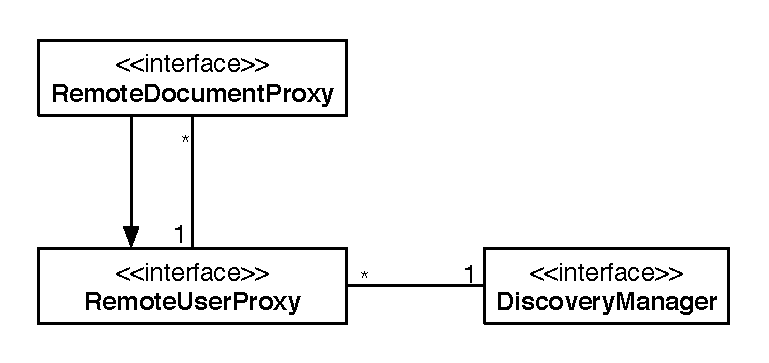
\includegraphics[width=4.90in,height=2.91in]{../images/finalreport/network_userManagement_uml.eps}
 }
 \caption{User Management}
 \label{fig:network.discovery.usermanagement}
\end{figure}

\paragraph{Interface exentions}
Types  \texttt{RemoteUserProxy}  and  \texttt{RemoteDocumentProxy} are extended for the network layer to provide an interface that allows modfications whereas the original interfaces are more 'getter-like' oriented since they are used by the upper layer as well.

 \texttt{RemoteUserProxyExt} adds methods mainly for the document management. The methods reflect the one-to-many relationship between user and document. Besides, state methods allow to indicate if a user was discovered by DNSSD or explicitly and if a \texttt{RemoteUserSession} for the user exists.

\begin{figure}[H]
 \centering
  \frame{
 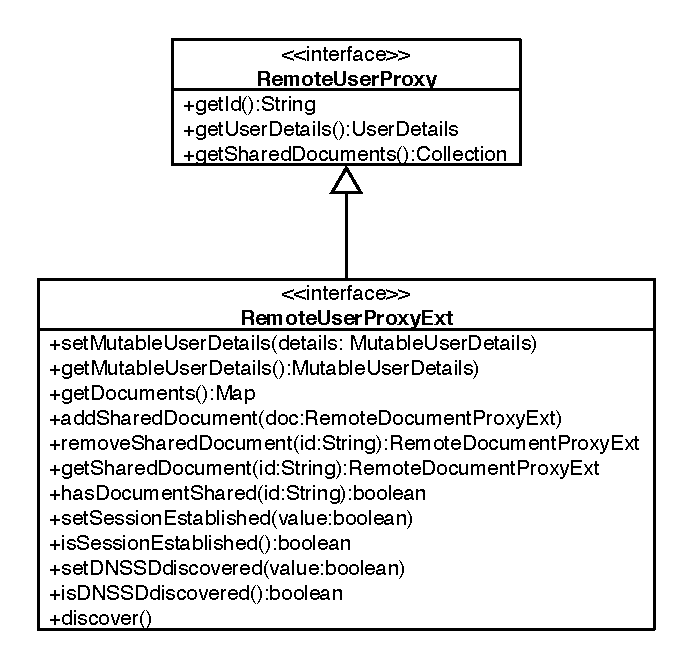
\includegraphics[width=5.50in,height=5.31in]{../images/finalreport/network_remoteUserProxyExt_uml.eps}
 }
 \caption{RemoteUserProxy and extension}
 \label{fig:network.discovery.remoteuserproxy.uml}
\end{figure}


\begin{figure}[H]
 \centering
  \frame{
 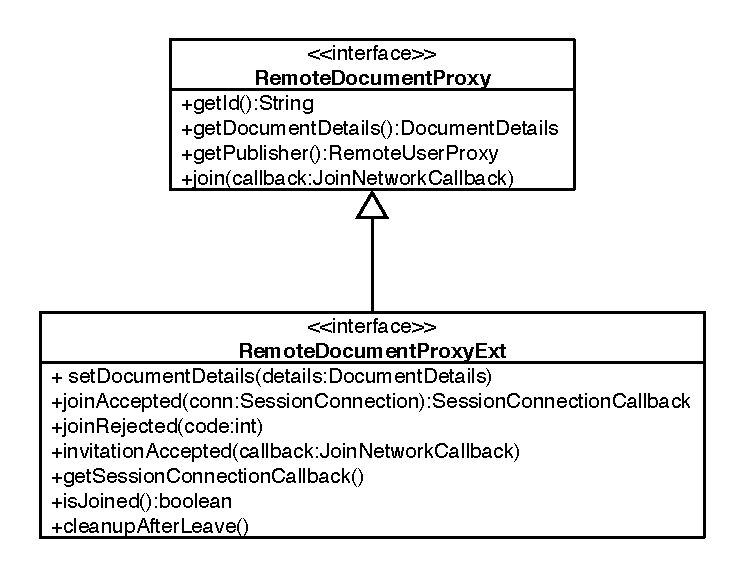
\includegraphics[width=5.85in,height=4.25in]{../images/finalreport/network_remoteDocumentProxyExt_uml.eps}
 }
 \caption{RemoteDocumentProxy and extension}
 \label{fig:network.discovery.remotedocumentproxy.uml}
\end{figure}

 \texttt{RemoteDocumentProxyExt} adds methods mainly for the join and invite use cases but also for updates of the document details. Method  \texttt{cleanupAfterLeave()} allows for a consistent object state since a document can be joined and left several times. So it is important to keep the object in one of two consistent states: Initialized and Joined.  

\begin{figure}[H]
 \centering
  \frame{
 \includegraphics[width=3.79in,height=3.40in]{../images/finalreport/network_remoteDocumentProxyExt_state.eps}
 }
 \caption{RemoteDocumentProxy State Diagram}
 \label{fig:network.discovery.remotedocumentproxy.state}
\end{figure}

\subsubsection{Network Connection Management}
Network Connection Management includes the session and connection handling for each remote user. For each user, there is one session of type (\texttt{RemoteUserSession}). This class is a wrapper around \texttt{TCPSession} from the BEEP API and provides further session management functions. For each session, there is one instance of \texttt{MainConnection}, through which most messages between peers are sent.

\begin{figure}[H]
 \centering
  \frame{
 \includegraphics[width=5.79in,height=4.79in]{../images/finalreport/network_sessionManagement_uml.eps}
 }
 \caption{Session Management for a Remote User}
 \label{fig:network.discovery.sessionmanagement}
\end{figure}

\paragraph{Connection}
A \texttt{AbstractConnection} represents a physical connection to a peer. It is basically a wrapper around a \texttt{Channel} provided by the BEEP API. All connection types traverse several states during their lifetime. This is depicted in the following figure.

\begin{figure}[H]
 \centering
  \frame{
 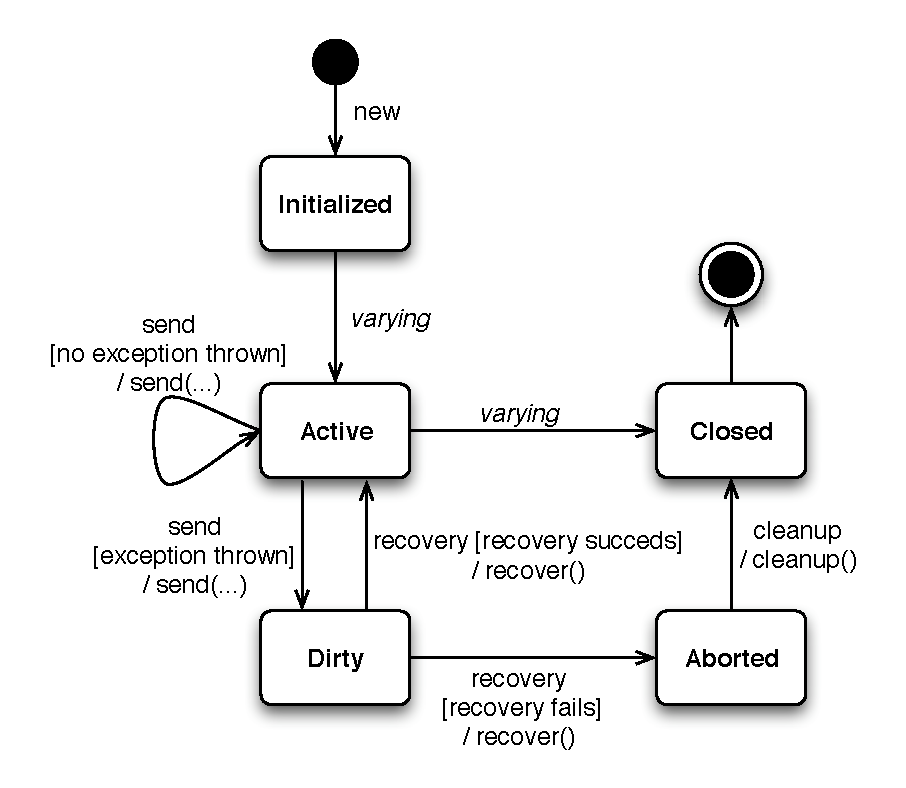
\includegraphics[width=5.82in,height=5.03in]{../images/finalreport/network_connection_state.eps}
 }
 \caption{State diagram for AbstractConnection}
 \label{fig:network.discovery.connection.state}
\end{figure}

There are tree different connection types which are explained below.

\begin{figure}[H]
 \centering
  \frame{
 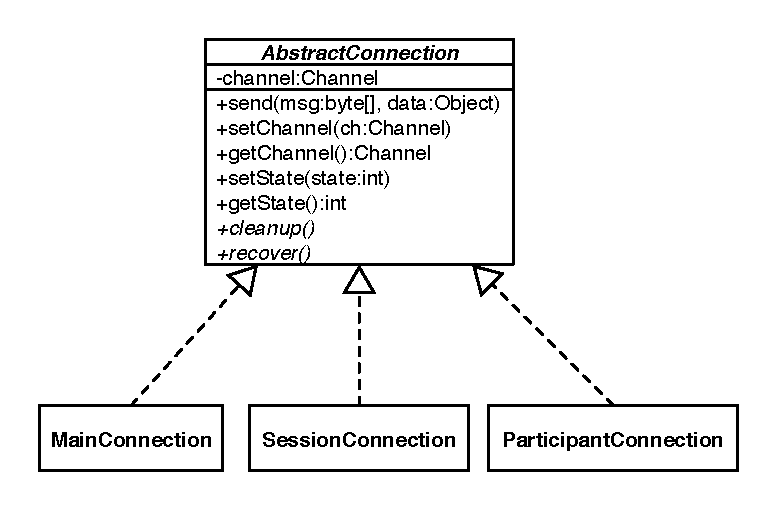
\includegraphics[width=5.82in,height=5.03in]{../images/finalreport/network_connection_uml.eps}
 }
 \caption{AbstractConnection Implementations}
 \label{fig:network.discovery.connection.uml}
\end{figure}


\subparagraph{MainConnection}
All basic communication except the document editing messages are sent with the \texttt{MainConnection}. It wraps a BEEP channel which represents the physical connection to the peer. Each user has only one instance of \texttt{MainConnection} and therefore only one channel for the main communication. Both peers use that same physical channel bidirectionally to communicate with each other (this property is provided by the BEEP framework). The main connection allows to send document management messages such as 'publish a document', 'invite user', 'join document' etc.

\subparagraph{SessionConnection}
The \texttt{SessionConnection} represents a physical connection starting from the local user to the session owner (publisher of document) in a collaborative editing session. Thus, \textt{SessionConnection}'s are only used by participants and not by the owner of a session. It allows a particpant to send session relevant messages to the session owner.

\subparagraph{ParticipantConnection}
The \textt{ParticipantConnection} represents a physical connection starting from the document session owner to a participant. Therefore, \textt{ParticipantConnection}'s are used only by session owners and not particpants. It allows a session owner to send relevant messages to the participants. 



\subsubsection{Connection Management}


If the local user acts as the publisher of a document and the remote user is a participant of that session, two \texttt{ParticipantConnection}'s to that user are established. If the local user acts as a participant of a document session, then two \texttt{SessionConnection}'s to the publisher of the documents are created (see next section for a detailed discussion). The \texttt{Session\-Manager} handles the creation and management of all \texttt{RemoteUserSession}'s. 


\subsubsection{Network Message Processing}

Request Filter Chain





\subsection{Implementation}
 \label{network.communication.implementation}


\subsubsection{Server Management}
Server management means the published document handling for the local user. The main 


\subsubsection{Remote User and Shared Documents Management}

\subsubsection{Network Connection Management}

\subsubsection{Processing of network messages}

\subsubsection{Session Management}

\subsubsection{Client and Server Specifics}


\subsection{Use Cases}



\subsection{Exception handling}

\subsection{Protocol}
